\documentclass[tikz,border=3mm]{standalone}
\usepackage{tikz}
\usetikzlibrary{arrows.meta,calc,patterns,decorations.pathmorphing}

\begin{document}
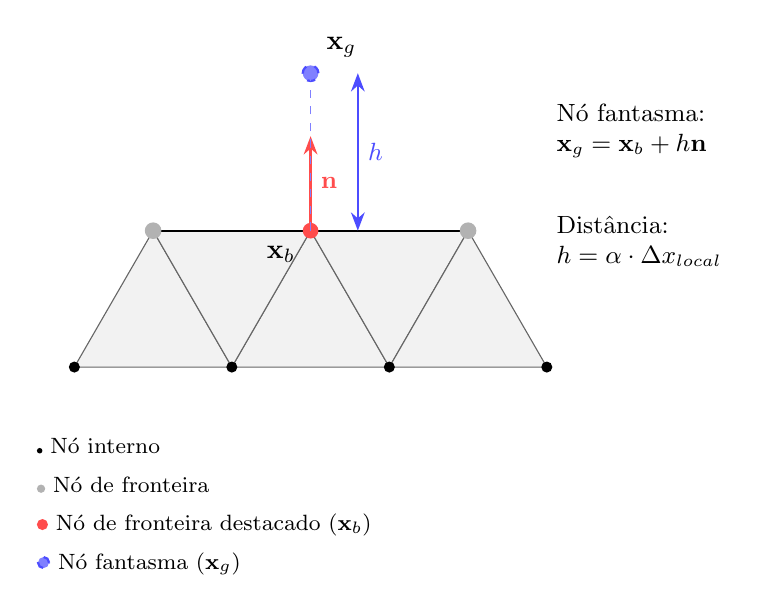
\begin{tikzpicture}[
    scale=2,
    >=Stealth,
    node/.style={circle,fill=black,inner sep=1.5pt},
    boundary node/.style={circle,fill=red!70,inner sep=2pt},
    ghost node/.style={circle,fill=blue!50,inner sep=2pt,draw=blue!70,thick,dashed},
    mesh edge/.style={black!60,thin},
    boundary edge/.style={black,thick},
    normal vector/.style={->,red!70,thick},
    dimension/.style={<->,blue!70,thick}
]

% Malha triangular de fundo (recorte)
% Triângulos do domínio (abaixo da fronteira)
\draw[mesh edge,fill=gray!10] (0,0) -- (1,0) -- (0.5,0.866) -- cycle;
\draw[mesh edge,fill=gray!10] (1,0) -- (2,0) -- (1.5,0.866) -- cycle;
\draw[mesh edge,fill=gray!10] (0.5,0.866) -- (1,0) -- (1.5,0.866) -- cycle;
\draw[mesh edge,fill=gray!10] (2,0) -- (2.5,0.866) -- (1.5,0.866) -- cycle;
\draw[mesh edge,fill=gray!10] (2,0) -- (3,0) -- (2.5,0.866) -- cycle;

% Aresta da fronteira (destacada) - NO TOPO
\draw[boundary edge] (0.5,0.866) -- (2.5,0.866);

% Nós da malha interna
\foreach \x/\y in {0/0, 1/0, 2/0, 3/0}
    \fill[black] (\x,\y) circle (1pt);

% Nós da fronteira (cinza)
\foreach \x/\y in {0.5/0.866, 2.5/0.866}
    \fill[gray!60] (\x,\y) circle (1.5pt);

% Nó de fronteira destacado (x_b) - AGORA NA FRONTEIRA SUPERIOR
\coordinate (xb) at (1.5,0.866);
\node[boundary node,label=below left:$\mathbf{x}_b$] at (xb) {};

% Vetor normal à fronteira (apontando para cima, para fora do domínio)
\coordinate (n_end) at ($(xb) + (0,0.6)$);
\draw[normal vector] (xb) -- (n_end) node[midway,right,font=\small] {$\mathbf{n}$};

% Nó fantasma (x_g) - NA DIREÇÃO NORMAL PARA FORA
\coordinate (xg) at ($(xb) + (0,1.0)$);
\node[ghost node,label=above right:$\mathbf{x}_g$] at (xg) {};

% Linha tracejada conectando x_b e x_g
\draw[blue!50,dashed,thin] (xb) -- (xg);

% Dimensão h
\draw[dimension] ($(xb) + (0.3,0)$) -- ($(xg) + (0.3,0)$) node[midway,right,font=\small] {$h$};

% Anotação explicativa
\node[anchor=west,font=\small,align=left] at (3,1.5) {
    Nó fantasma:\\
    $\mathbf{x}_g = \mathbf{x}_b + h\mathbf{n}$
};

\node[anchor=west,font=\small,align=left] at (3,0.8) {
    Distância:\\
    $h = \alpha \cdot \Delta x_{local}$
};

% Legenda
\node[anchor=west,font=\footnotesize] at (-0.3,-0.5) {
    \tikz{\fill[black] circle (1pt);} Nó interno
};
\node[anchor=west,font=\footnotesize] at (-0.3,-0.75) {
    \tikz{\fill[gray!60] circle (1.5pt);} Nó de fronteira
};
\node[anchor=west,font=\footnotesize] at (-0.3,-1.0) {
    \tikz{\fill[red!70] circle (2pt);} Nó de fronteira destacado ($\mathbf{x}_b$)
};
\node[anchor=west,font=\footnotesize] at (-0.3,-1.25) {
    \tikz{\fill[blue!50,draw=blue!70,dashed,thick] circle (2pt);} Nó fantasma ($\mathbf{x}_g$)
};

\end{tikzpicture}
\end{document}
